\paragraph{Units.} Every budget is counted in \emph{units}. For LENGTH and $\SMK$ (Definitions~\ref{def:greedy}
and~\ref{def:smk}) a unit is one \emph{expansion}: remove the first state from the heap, generate its S-move children,
drop those already discovered and push the rest onto the heap by priority. The CoV used here (Section~\ref{sec:cov}) is
one-shot: it is applied once, to the starting presentation, before any search, and builds new presentations, which
LENGTH then searches. Building them costs no units. For the hybrid (Definition~\ref{def:hybrid}) a unit is one
expansion of its search or one S-move of its finishing checks. A budget is per
presentation, a failed search is charged all of it, and path lengths are counted in S-moves (for the hybrid, S-moves plus Nielsen images).

\paragraph{Time per unit.} A pop does different work in each method: LENGTH and $\SMK$ differ in the priority they
compute, the hybrid also builds Nielsen images and runs finishing checks, and CoV creates images instead of S-move
children. Equal budgets in units are a fair comparison only if a unit costs about the same in each method, so we time
one pop of each method on the same states. On each test state, each method starts a fresh search, so the heap holds
only that state, and makes one pop: it removes the state, creates all its children, discards those already discovered,
computes the priorities of the rest and pushes them onto the heap. The test states are drawn at random from the states
that LENGTH and $\SMK$ popped on MS640 with a budget of $10^4$ units, up to $60$ per range of total length $\lambda$,
and every method is timed on the same states. All run in pure Python (one core, Intel Xeon $2.1$ GHz, best of five
runs).
\begin{center}
\small
\begin{tabular}{lrrrrr}
\toprule
$\lambda$ & states & LENGTH & $\SMK$ & hybrid & CoV\\
\midrule
$\le10$ & $46$ & $0.12$ & $0.14$ & $0.28$ & $0.25$\\
$11$--$15$ & $60$ & $0.85$ & $1.05$ & $1.37$ & $3.24$\\
$16$--$20$ & $60$ & $1.61$ & $2.00$ & $3.03$ & $6.05$\\
$21$--$25$ & $60$ & $2.99$ & $3.41$ & $10.08$ & $11.23$\\
$\ge26$ & $60$ & $4.66$ & $6.00$ & $6.85$ & $16.47$\\
\midrule
mean & & $2.04$ & $2.52$ & $4.32$ & $7.45$\\
relative to LENGTH & & $1$ & $1.23$ & $2.11$ & $3.64$\\
\bottomrule
\end{tabular}

\smallskip
\footnotesize Time of one pop in ms, averaged over the states of the row. The mean row averages the five rows; the last row divides it by the LENGTH mean.
\end{center}
For example, one pop of $\mathrm{AK}(3)$ ($\lambda=13$) takes $0.69$ ms for LENGTH, $0.87$ ms for $\SMK$, $1.17$ ms
for the hybrid and $2.61$ ms for CoV. A longer state has more children, so its pop costs more. An $\SMK$ pop differs
from a LENGTH pop only in its priority and costs $1.1$--$1.3$ times as much. A hybrid pop also builds the four Nielsen
images and runs the finishing checks, and costs $1.5$--$3.4$ times as much; its other units are single moves and cost
less. A CoV pop costs $3.5$--$3.8$ LENGTH pops for $\lambda>10$, but CoV makes it only once, on the starting
presentation, which is why it is not charged. A unit of each method thus costs within a small factor of one LENGTH
expansion, and equal budgets in units are comparable up to that factor.

\subsection{AC search methods}\label{sec:methods}

The three methods below are AC search methods: each solve comes with an AC certificate. All three search over
S-moves; LENGTH and $\SMK$ use nothing else.

\begin{definition}[S-move and state]\label{def:smove}
For a cyclically reduced word $r$ and $0\le k<|r|$, let $\rot_k(r)$ be $r$ with its last $k$ letters moved to the
front. A \emph{substitution move} (S-move) $(i,j,s,k_1,k_2)$, with $i\neq j$, $s=\pm1$ and the last letter of $\rot_{k_1}(r_i)$ inverse to the first letter of
$\rot_{k_2}(r_j^{\,s})$, replaces
\[
r_i\;\longmapsto\;\rot_{k_1}(r_i)\cdot\rot_{k_2}\!\big(r_j^{\,s}\big)
\]
and cyclically reduces \cite{FTS26}. A \emph{state} is a presentation up to rotation and inversion of each relator and permutation of the relators,
stored in a canonical form described in \cite{FTS26}.
\end{definition}

\begin{definition}[Greedy search]\label{def:greedy}
A greedy search with priority $\pi$, budget $B$ and length bound $c$ keeps a heap of states, lowest $\pi$ first,
starting from the input. An \emph{expansion} removes the first state $Q$: if every relator of $Q$ has length $1$, $Q$
is solved; otherwise the children of $Q$ under S-moves that are new and have every relator of length at most $c$ are pushed onto the heap. The search stops after $B$ pops, and the certificate is the chain of parent moves. Ties in $\pi$ are broken by depth and then by a fixed order on states described in \cite{FTS26}, so every run is deterministic.
\end{definition}

The two greedy searches below differ only in the priority, that is, in which state they expand next.

\begin{definition}[LENGTH]\label{def:length}
\emph{LENGTH} is the greedy search with $\pi=\lambda$, the total length: it always expands a shortest state. It is the
greedy search of \cite{SMM24}.
\end{definition}

\begin{definition}[$\SMK$]\label{def:smk}
Read each relator cyclically. A \emph{block} is a maximal run of letters of one generator, $x$ and $x^{-1}$ counted
alike. For a state $Q$:
\begin{itemize}
  \item $\mathrm{MK}(Q)$ is the largest number of $x$-blocks or of $y$-blocks in a single relator of $Q$ (a relator
  that is a power of one generator counts $0$);
  \item $S(Q)$ is the mean length of the $x$-blocks or of the $y$-blocks, pooled over both relators, whichever is
  smaller (a generator that does not occur is ignored).
\end{itemize}
$\SMK$ is the greedy search with
\[
\pi_{\SMK}(Q)=\lambda(Q)+20\,S(Q)+2\,\mathrm{MK}(Q).
\]
\end{definition}

\begin{example}
Take $\mathrm{AK}(3)=\pres{x,y}{x^3y^{-4},\ xyxy^{-1}x^{-1}y^{-1}}$. The first relator has the blocks
$x^3\mid y^{-4}$, one of each generator; the second has the six blocks $x\mid y\mid x\mid y^{-1}\mid x^{-1}\mid y^{-1}$,
three of each. Hence $\mathrm{MK}=3$. The $x$-blocks have lengths $3,1,1,1$, mean $1.5$, and the $y$-blocks
$4,1,1,1$, mean $1.75$, so $S=1.5$. With $\lambda=13$,
\[
\pi_{\SMK}(\mathrm{AK}(3))=13+20\cdot1.5+2\cdot3=49,\qquad \pi_{\mathrm{LENGTH}}(\mathrm{AK}(3))=13.
\]
\end{example}

\begin{remark}[Choice of $S$ and $\mathrm{MK}$]
The features $S$ and $\mathrm{MK}$ come from comparing, on the starting presentations of MS1190, the $640$ rows that
LENGTH solves with the $550$ it does not, and keeping the features that best separate the two groups. They are
imperfect: no feature of a single state can decide whether a presentation is easy or hard. For example,
\[
\pres{x,y}{y^{-1}x^{-1}yxy^{-1}x,\ y^{-4}x^3}
\qquad\text{and}\qquad
\pres{x,y}{y^{-1}x^{-1}y^{-1}xyx,\ y^{-4}x^3}
\]
have the same $\lambda=13$, $\mathrm{MK}=3$ and $S=1.5$, hence the same $\pi_{\SMK}=49$. LENGTH solves the first in
$107$ expansions, with a path of $19$ S-moves, while the second is $\mathrm{AK}(3)$. For example, length is also an imperfect heuristic, but the idea here is to obtain features that represent a state that might be easier to solve on average so that temporarily increasing the length can be a possibility.
\end{remark}

\begin{definition}[Hybrid solver]\label{def:hybrid}
The input is a balanced presentation $P$ of rank $2$ with $|\det M|=1$, where $M$ is the $2\times2$ matrix of exponent
sums of the relators, and the \emph{Nielsen maps} are
$x\mapsto xy^{\pm1}$ and $y\mapsto yx^{\pm1}$. The solver has two parts (Figure~\ref{fig:hybrid}).
\begin{enumerate}
  \item \emph{Finishing checks.} Two shapes are finished directly by S-moves. (i) A generator occurs once in a relator
  (Proposition~\ref{prop:once}). (ii) A relator
  reads cyclically as $g^ah^pg^{-a}h^q$ and its pinch replacements bring the other relator to at most one $g$-block
  (Proposition~\ref{prop:pinch}).
  \item \emph{Search.} If the checks do not finish $P$, a best-first search with priority $\lambda$, on states taken
  up to signed permutations of the generators. The children of a state are its S-move children and its four Nielsen images. Every new child goes through two filters that change nothing
  (Definition~\ref{def:filters}); a child that passes goes to the check they name, which then finishes it
  (Proposition~\ref{prop:filters}). The other children are pushed onto the heap.
\end{enumerate}
The \emph{units} of a run are its pops, plus one for every S-move that a check applies.
\end{definition}

\begin{figure}[ht]
\centering
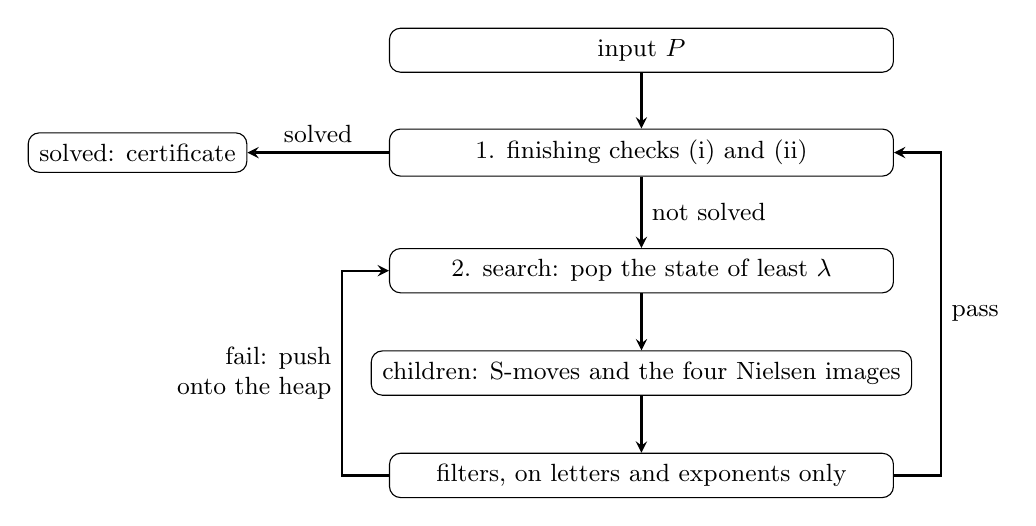
\begin{tikzpicture}[x=1cm,y=1cm,font=\small,
  box/.style={draw,rounded corners,align=center,inner sep=4pt,minimum width=6.4cm},
  arr/.style={->,>=stealth,thick}]
  \node[box] (in) at (0,0) {input $P$};
  \node[box] (fin) at (0,-1.3) {1. finishing checks (i) and (ii)};
  \node[draw,rounded corners,inner sep=4pt] (out) at (-6.4,-1.3) {solved: certificate};
  \node[box] (pop) at (0,-2.8) {2. search: pop the state of least $\lambda$};
  \node[box] (kids) at (0,-4.1) {children: S-moves and the four Nielsen images};
  \node[box] (filt) at (0,-5.4) {filters, on letters and exponents only};
  \draw[arr] (in) -- (fin);
  \draw[arr] (fin.west) -- node[above]{solved} (out);
  \draw[arr] (fin) -- node[right]{not solved} (pop);
  \draw[arr] (pop) -- (kids);
  \draw[arr] (kids) -- (filt);
  \draw[arr] (filt.west) -- ++(-0.6,0) |- node[pos=0.25,left,align=right]{fail: push\\onto the heap} (pop.west);
  \draw[arr] (filt.east) -- ++(0.6,0) |- node[pos=0.25,right,align=left]{pass} (fin.east);
\end{tikzpicture}
\caption{The hybrid solver. A child that passes the filters goes to the finishing checks, which then finish it; the
other children are pushed onto the heap.}
\label{fig:hybrid}
\end{figure}

The hybrid stays at rank $2$, so its certificates are AC paths. It can also change the rank during the search
(Section~\ref{sec:hybrid}); that extension is left out here.

\paragraph{Scores.} We compare the three methods at equal budgets in units: the number of
presentations each solves on the three benchmarks.

\begin{center}
\small
\begin{tabular}{llrrrrr}
\toprule
& & \multicolumn{5}{c}{budget (units)}\\
\cmidrule(lr){3-7}
benchmark & method & $10^3$ & $10^4$ & $10^5$ & $10^6$ & $10^7$\\
\midrule
MS640 & LENGTH & $554$ & $606$ & $634$ & $640$ & $640$\\
(of $640$) & $\SMK$ & $574$ & $626$ & $640$ & $640$ & $640$\\
& dual, single CoV & $593$ & $621$ & $640$ & $640$ & $640$\\
& dual, auto CoV & $614$ & $634$ & $640$ & $640$ & $640$\\
& triple$^{\dagger}$ & $612$ & $634$ & $640$ & $640$ & $640$\\
& hybrid & $640$ & $640$ & $640$ & $640$ & $640$\\
\midrule
bench60 & LENGTH & $29$ & $40$ & $54$ & $60$ & $60$\\
(of $60$) & $\SMK$ & $37$ & $52$ & $60$ & $60$ & $60$\\
& dual, single CoV & $43$ & $52$ & $60$ & $60$ & $60$\\
& dual, auto CoV & $51$ & $56$ & $60$ & $60$ & $60$\\
& triple$^{\dagger}$ & $49$ & $56$ & $60$ & $60$ & $60$\\
& hybrid & $60$ & $60$ & $60$ & $60$ & $60$\\
\midrule
ladder100 & LENGTH & $11$ & $20$ & $40$ & $60$ & $80$\\
(of $100$) & $\SMK$ & $23$ & $53$ & $69$ & $87$ & $91$\\
& dual, single CoV & $56$ & $82$ & $100$ & $100$ & $100$\\
& dual, auto CoV & $77$ & $96$ & $100$ & $100$ & $100$\\
& triple$^{\dagger}$ & $81$ & $97$ & $100$ & $100$ & $100$\\
& hybrid & $99$ & $100$ & $100$ & $100$ & $100$\\
\bottomrule
\end{tabular}

\smallskip
\footnotesize Dual and triple: the greedy searches of ACSolverES (E.~Steffen), with the CoV work counted in
substitution-pop units. Counted in nodes, where a CoV pop counts as $1$, the $10^3$ / $10^4$ columns read: single CoV
$604$/$627$, $46$/$52$, $64$/$92$; auto CoV $618$/$634$, $51$/$56$, $80$/$97$; triple $618$/$634$, $51$/$56$,
$86$/$97$. Every row is solved within $10^5$, so the $10^6$ and $10^7$ columns are full.
$^{\dagger}$The triple's complete CoV is not an automorphism, so $54$, $7$ and $17$ of its solves prove only stable
AC-triviality.
\end{center}

$\SMK$ solves all of MS640 and bench60 by $10^5$ units, LENGTH only by $10^6$. On ladder100 neither finishes by
$10^7$: $9$ rows are unsolved by both. The hybrid solves all of MS640 and bench60 at $10^3$ units and all of
ladder100 at $10^4$; its hardest row, \texttt{ac19\_70845}, takes $2{,}267$ units.

\paragraph{Units and path lengths.} For every solve we also record the units it took and the length of its path:
S-moves, and for the hybrid S-moves plus Nielsen images.

\begin{center}
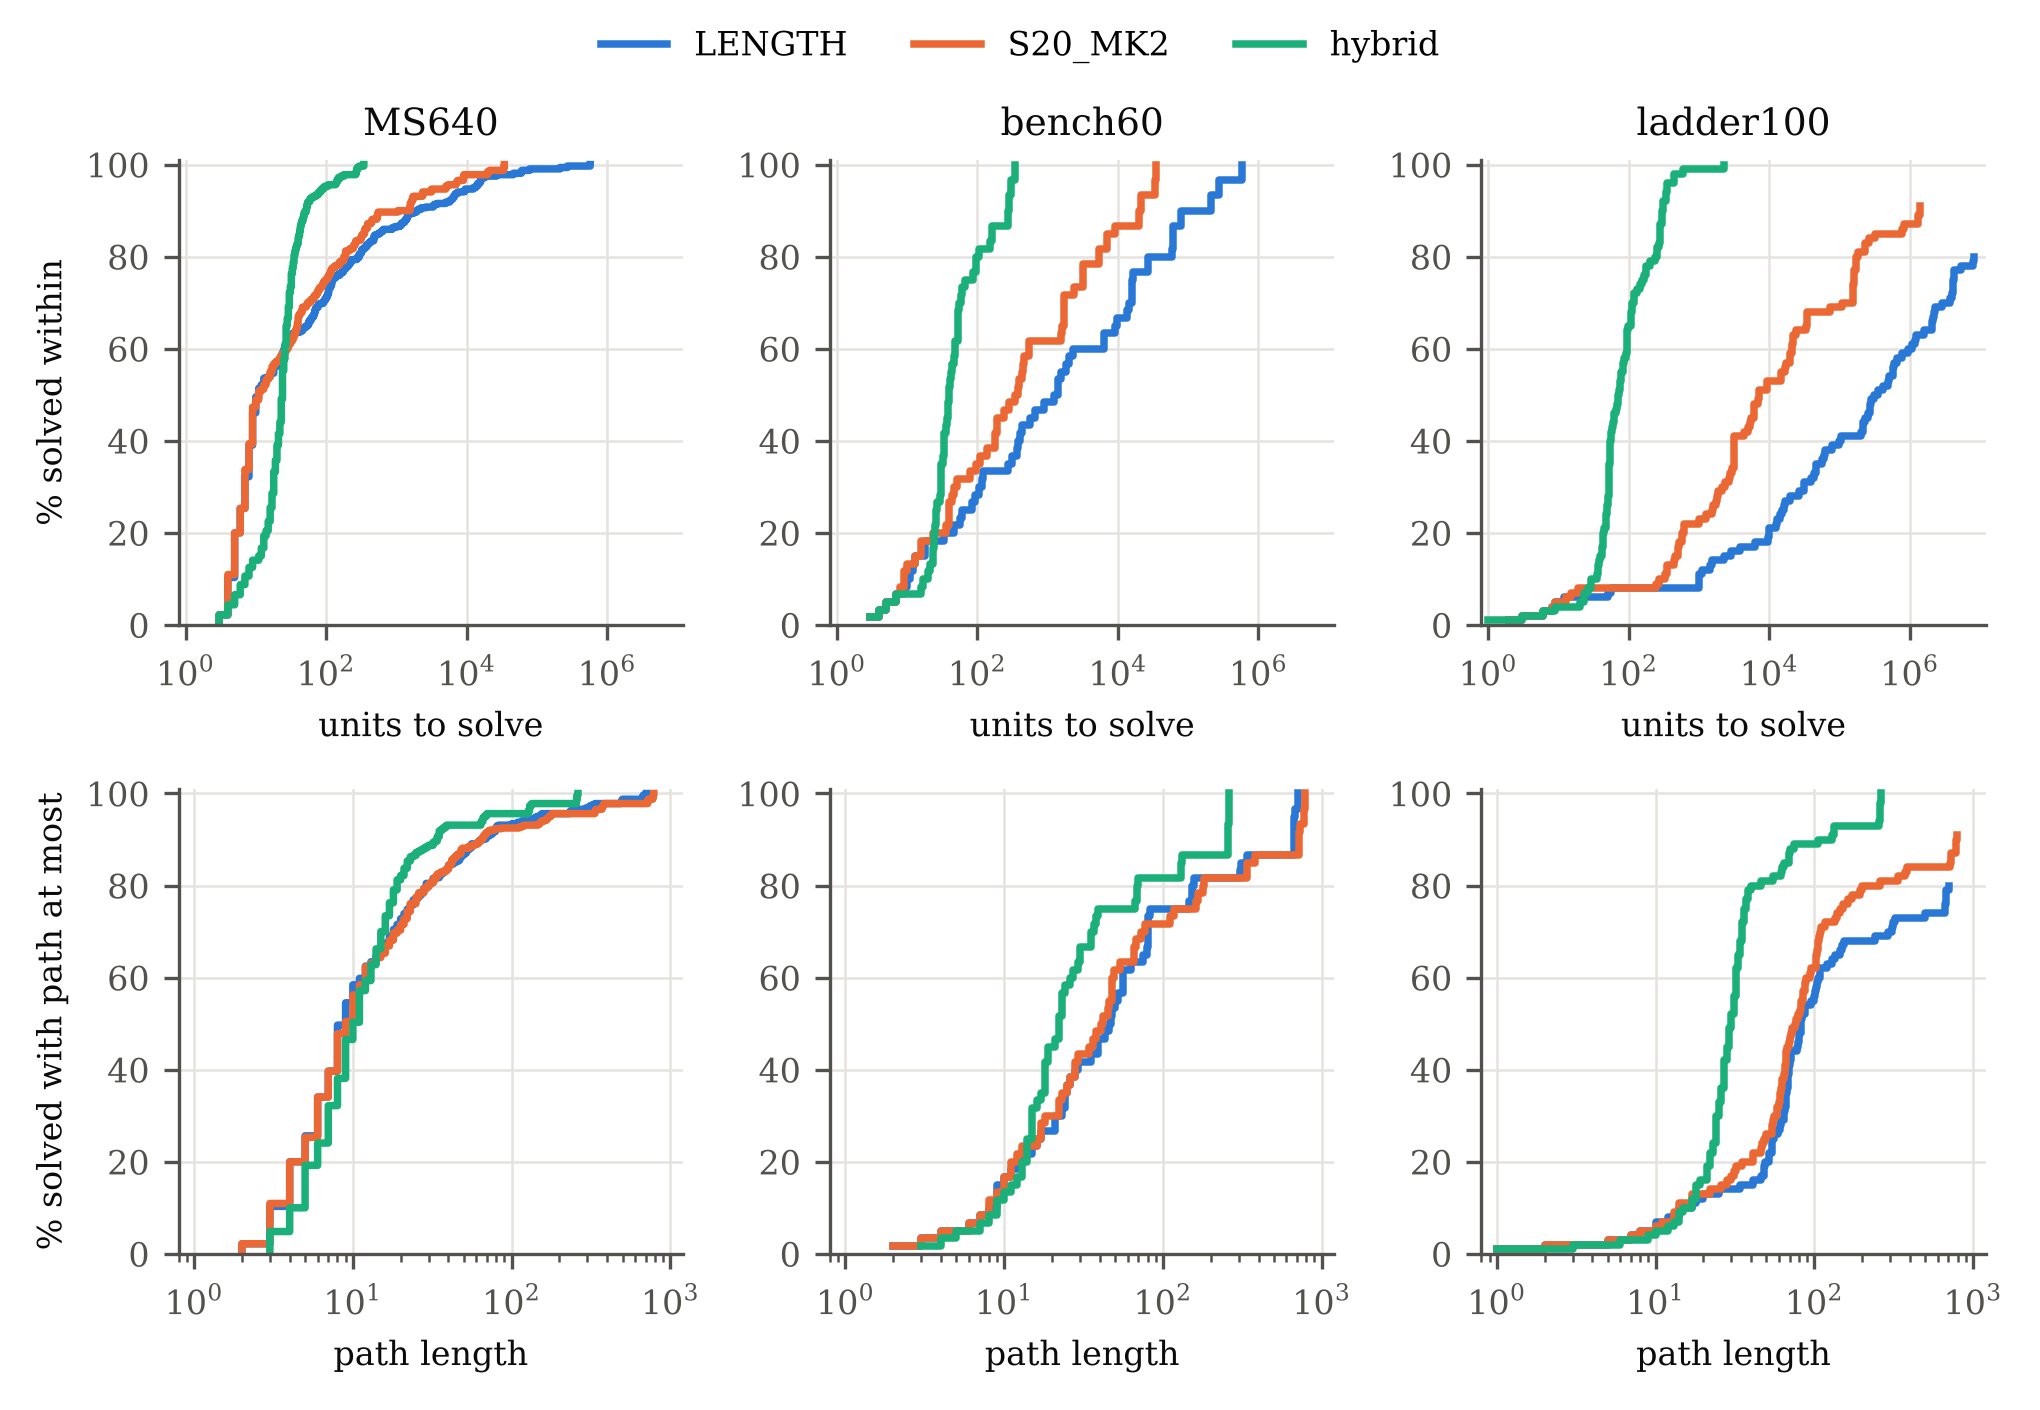
\includegraphics[width=\textwidth]{figures/units_paths.png}
\end{center}

\begin{center}
\small
\begin{tabular}{llrrrrrr}
\toprule
& & \multicolumn{3}{c}{units to solve} & \multicolumn{3}{c}{path length}\\
\cmidrule(lr){3-5}\cmidrule(lr){6-8}
benchmark & method & mean & median & max & mean & median & max\\
\midrule
MS640 & LENGTH & $4{,}963$ & $11$ & $574{,}959$ & $36.8$ & $9$ & $708$\\
 & $\SMK$ & $995$ & $11$ & $34{,}438$ & $42.9$ & $9$ & $787$\\
 & dual, single CoV & $729$ & $31$ & $25{,}854$ & $40.8$ & $10$ & $825$\\
 & dual, auto CoV & $349$ & $14$ & $18{,}110$ & $44.0$ & $9$ & $939$\\
 & triple$^{\dagger}$ & $376$ & $22$ & $18{,}745$ & $44.1$ & $9$ & $939$\\
 & hybrid & $23$ & $11$ & $322$ & $21.2$ & $10$ & $262$\\
\midrule
bench60 & LENGTH & $45{,}244$ & $1{,}311$ & $574{,}959$ & $142.6$ & $47$ & $708$\\
 & $\SMK$ & $4{,}685$ & $359$ & $34{,}438$ & $154.3$ & $42$ & $787$\\
 & dual, single CoV & $3{,}509$ & $326$ & $25{,}582$ & $148.0$ & $45$ & $780$\\
 & dual, auto CoV & $1{,}795$ & $192$ & $18{,}079$ & $161.8$ & $39$ & $939$\\
 & triple$^{\dagger}$ & $1{,}879$ & $198$ & $18{,}637$ & $161.7$ & $39$ & $939$\\
 & hybrid & $67$ & $28$ & $322$ & $59.9$ & $22$ & $262$\\
\midrule
ladder100 & LENGTH & $975{,}165$ & $101{,}771$ & $8{,}204{,}360$ & $130.8$ & $69$ & $706$\\
 & $\SMK$ & $114{,}830$ & $6{,}073$ & $1{,}383{,}279$ & $133.9$ & $69$ & $787$\\
 & dual, single CoV & $4{,}654$ & $796$ & $61{,}821$ & $114.7$ & $58$ & $780$\\
 & dual, auto CoV & $1{,}523$ & $315$ & $18{,}113$ & $122.2$ & $58$ & $939$\\
 & triple$^{\dagger}$ & $1{,}373$ & $314$ & $18{,}680$ & $121.2$ & $54$ & $939$\\
 & hybrid & $127$ & $53$ & $2{,}267$ & $49.7$ & $30$ & $262$\\
\bottomrule
\end{tabular}

\smallskip
\footnotesize Over the rows each method solves (on ladder100: $80$, $91$, all $100$ for the dual and triple
searches, and $100$). Dual and triple: units count the CoV work in substitution-pop units, and a path counts each CoV
move as one step (a map $x\mapsto xy^k$ counts $1$). $^{\dagger}$Stable AC certificate on $54$, $7$ and $17$ of the
rows.
\end{center}


On easy rows the hybrid spends about as many units as the greedy searches (median $11$ against $11$ on MS640); on
hard rows it needs far fewer, at most $2{,}267$ against $8.2$ million for LENGTH.
Its paths are shorter on hard rows too: on the $80$ ladder100 rows that all three solve, $53.8$ steps on average
against $130.8$ for LENGTH and $142.4$ for $\SMK$. $\SMK$ paths are about as long as LENGTH's.
